\section*{Objetivos}

A continuación, se muestra el objetivo a lograr con la elaboración de esta tarea:
\begin{itemize}
    \item Identificar componentes del sistema de control de lazo cerrado en un caso
de aplicación y la simulación básica del sistema de control realimentado.
\end{itemize}

\section*{Parte 1}

\hspace{1.27cm} En la \hyperref[fig1]{Figura 1} se muestra el esquema de control implementado por un laboratorio farmacéutico para controlar el nivel de pH en un antibiótico y mantenerlo en un valor de 8.
El pH es una medida del nivel de acidez o alcalinidad de una solución acuosa y se suele medir a una temperatura de referencia de \SI{25}{\celsius}, por lo cual se procura tener el cuarto de laboratorio bajo dichas condiciones ambientales al hacer mediciones de dicha variable. 
Es importante recordar que al disminuir el valor del pH se incrementa la acidez de una sustancia. 
El nivel de pH en el tanque se mide utilizando un medidor de pH (phímetro), el cual es un dispositivo que genera un nivel de tensión directa, relacionado linealmente con el nivel de pH tal y como se observa en la figura 2. 
Dicho nivel de tensión es procesado por un transmisor que envía una señal de corriente de 4 mA a 20 mA al controlador.

\hspace{1.27cm} De acuerdo con la \hyperref[fig1]{Figura 1}, al tanque ingresan dos sustancias: Una solución A y una solución B. 
La solución A es una sustancia conocida como base y la cantidad de dicha sustancia que se agrega al tanque puede variar según su disponibilidad y también debido a la demanda de producción del antibiótico. 
Para variar la cantidad de la solución A se utiliza la válvula 1 de apertura manual. Por otro lado, al regular la cantidad de la sustancia B (un ácido) se controla el nivel de pH del antibiótico en el tanque, con lo que, si se agregara más de esta solución al tanque, se disminuiría el pH del antibiótico. 
La apertura de la válvula de salida suele ser constante, sin embargo, podría variarse (utilizando la válvula 2 de apertura manual) dependiendo de la demanda de producción del antibiótico.

\begin{itemize}
    \item (40 puntos) Dibuje un diagrama de bloques completo del proceso y su sistema de control, describiendo todas las variables físicas y las señales involucradas en él. 
        Indique y describa dos posibles perturbaciones para este sistema de control según la definición de la variable controlada.
\end{itemize}

\begin{figure}[!h]
    \centering
    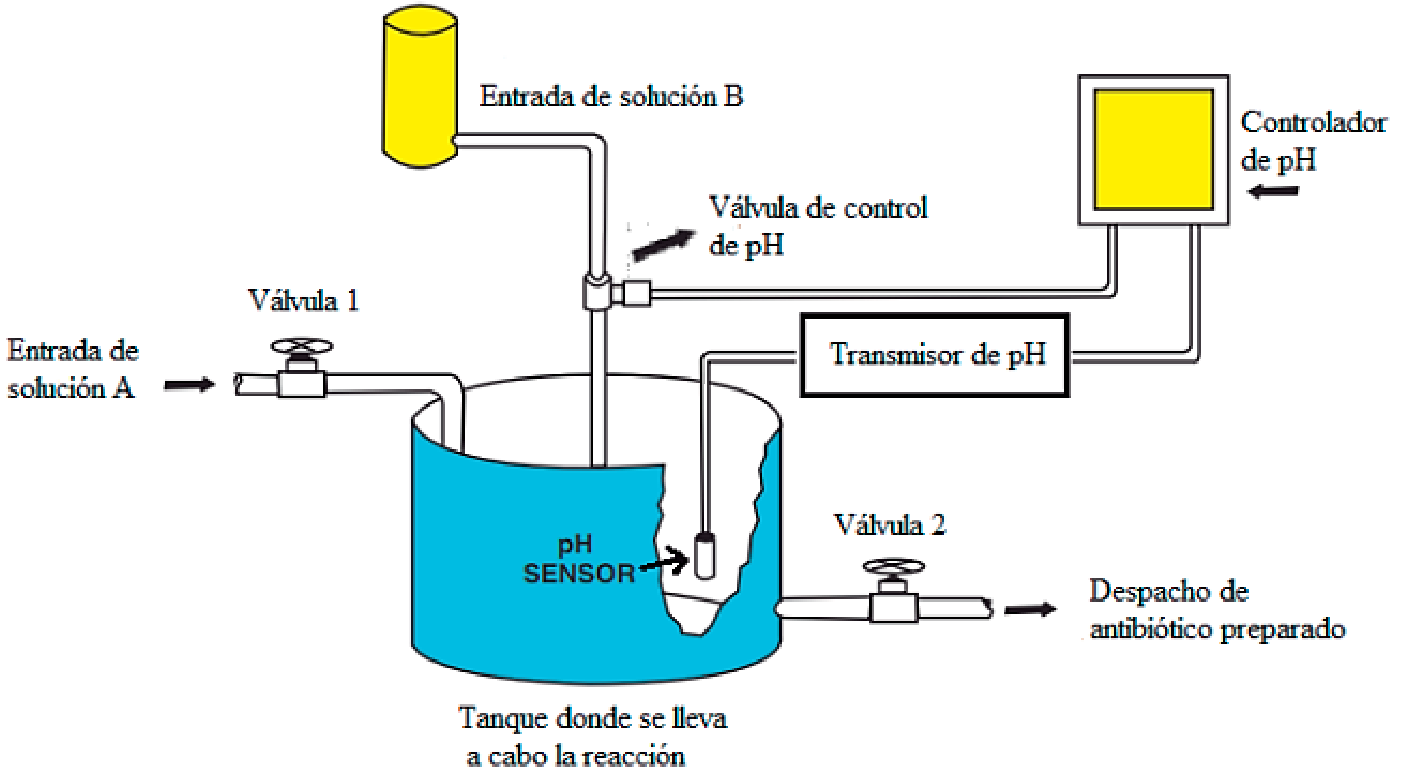
\includegraphics[width = 0.5\linewidth]{figs/fig1.png}
    \caption{Sistema de control de pH}
    \label{fig1}
\end{figure}

\pagebreak

\textit{Solución.} Considere el siguiente diagrama de bloques del proceso:

\begin{figure}[!h]
    \centering
    \tikzstyle{block} = [draw, fill=white, rectangle, 
    minimum height=3em, minimum width=4em, node distance=2cm]
    \tikzstyle{gain} = [draw, fill=white, rectangle, 
    minimum height=3em, minimum width=2em, node distance=2cm]
    \tikzstyle{sum} = [draw, fill=white, circle, minimum size=15pt, node distance=2cm]
    \tikzstyle{input} = [coordinate]
    \tikzstyle{output} = [coordinate]
    \tikzstyle{pinstyle} = [pin edge={to-,thin,black}]
    \begin{tikzpicture}[auto, node distance=3cm]
        
        %nodos
        \node [input, name=input]{};
        \node [gain, right of=input, xshift=-2em](gain){$K_r$};
        \node [sum, right of=gain, xshift=0.5em] (sum1) {};
        \node [block, right of=sum1](mcu){$C(s)$};
        \node [block, right of=mcu, xshift=2em](actuador){$G_B(s)$};
        \node [sum, right of=actuador, xshift=1em](sum2){};
        \node [block, right of=sum2, xshift=2em](proceso){$G_P(s)$};
        \node [sum, right of=proceso, xshift=1em](sum3){};
        \node [block, below of=proceso](sensor){$G_s(s)$};
        \node [sum, below of=sum2](sum4){};
        \node [block, below of=actuador](transmisor){$G_t(s)$};
        \node [sum, below of=mcu](sum5){};
        \node [output, right of=sum3, xshift=-3.5em](output){};
        \node [input, below of=sum4, yshift=3em](ruidos){};
        \node [input, below of=sum5, yshift=3em](ruidot){};
        \node [block, above of=sum2, yshift=1em](gddp){$G _{dp}(s)$};       
        \node [block, above of=sum3, yshift=1em](gt){$G_T(s)$};       
        \node [input, right of=gddp, xshift=-2em](ddp){};    
        \node [input, left of=gt, xshift=2em](dt){};

        %señales
        \draw [-{Latex}] (input) node[name=r, left]{$r(s)$} -- (gain);
        \draw [-{Latex}] (gain) -- (sum1) node[name=rma, midway, above]{$r ^{\prime}(s)$};
        \draw [-{Latex}] (sum1) -- (mcu) node[name=e, midway, above]{$e(s)$};
        \draw [-{Latex}] (mcu) -- (actuador) node[name=u, midway, above]{$u(s)$};
        \draw [-{Latex}] (actuador) -- (sum2) node[name=m, midway, above]{$m(s)$};
        \draw [-{Latex}] (sum2) -- (proceso) node[name=mm, midway, above]{$m ^{\prime}(s)$};
        \draw [-{Latex}] (proceso) -- (sum3) node[name=cc, midway, above]{$c ^{\prime}(s)$};
        \draw [-{Latex}] (sum3) -- (output) node[name=c, midway, above]{$c(s)$};
        \draw [-{Latex}] (c) -- (c|-sensor) -- (sensor);
        \draw [-{Latex}] (sensor) -- (sum4) node[name=yss, midway, above]{$y_s ^{\prime}(s)$};
        \draw [-{Latex}] (sum4) -- (transmisor) node[name=ys, midway, above]{$y_s(s)$};
        \draw [-{Latex}] (transmisor) -- (sum5) node[name=ytt, midway, above]{$y _{t}(s)$};
        \draw [-{Latex}] (sum5) -- (sum1|-sum5) node[name=y, midway, above]{$y(s)$} -- (sum1);
        \draw [-{Latex}] (ruidos) node[name=ns, below]{$n_s(s)$} -- (sum4) ;
        \draw [-{Latex}] (ruidot) node[name=nt, below]{$n_t(s)$} -- (sum5); 
        \draw [-{Latex}] (ddp) -- (gddp) node[name=disp, midway, above]{$d _{dp}(s)$};
        \draw [-{Latex}] (gddp) -- (sum2) node[name=dddp, midway, left]{$d _{dp} ^{\prime}(s)$};
        \draw [-{Latex}] (dt) -- (gt) node[name=temp, midway, above]{$d _{t}(s)$};
        \draw [-{Latex}] (gt) -- (sum3) node[name=dddt, midway, left]{$d _{t} ^{\prime}(s)$};

        %simbolos extra (+zzipo de nodo, posición](nombre){label};
        \node [below right=-4pt of sum5]{$+$};
        \node [above right=-4pt of sum5]{$+$};
        \node [below right=-4pt of sum4]{$+$};
        \node [above right=-4pt of sum4]{$+$};
        \node [below right=-4pt of sum4]{$+$};
        \node [below left=-4pt of sum1]{$-$};
        \node [above left=-4pt of sum1]{$+$};
        \node [above right=-4pt of sum2]{$+$};
        \node [below left=-4pt of sum2]{$+$};
        \node [above right=-4pt of sum3]{$+$};
        \node [below left=-4pt of sum3]{$+$};
    \end{tikzpicture}
    \caption{Diagrama de bloques del sistema de control de pH}
    \label{fig2}
\end{figure}



A continuación, se muestra un conjunto de tablas que describen las funciones de transferencia, señales, y, perturbaciones y ruido, que conforman el sistema de control realimentado representado por medio del diagrama de bloques elaborado anteriormente.

\begin{figure}[!h]
    \centering
    \setlength\extrarowheight{3mm}
    \begin{tabular}{p{3cm}p{3cm}p{10cm}}
        \toprule\\[-2.5em]
        Abreviación & Clasificación & Descripción\\
        \midrule
        $K_r$ & Ganancia & Convierte el valor de referencia a una corriente a partir de una escala conocida\\
        $C(s)$ & Controlador & En base al error, controla el pH del líquido en el tanque por medio de una señal de control\\
        $G_B(s)$ & Actuador/ \newline Elemento final de control & En base a la señal de control, modifica el porcentaje de apertura de la válvula de control de pH para modificar el caudal de la sustancia B\\
        $G_P(s)$ & Proceso & Tanque con solución acuosa, cuyo pH es modificado en base al caudal de sustancia ácida/alkalina que le ingrese\\
        $G_S(s)$ & Sensor & pHímetro, que convierte el nivel de pH a una señal de tensión DC\\
        $G_t(s)$ & Transmisor & Convierte una señal de tensión DC correspondiente al nivel de pH, a una señal de corriente\\
        \bottomrule
    \end{tabular}
    \caption{Funciones de transferencia del sistema de control realimentado}
    \label{t2}
\end{figure}


\pagebreak
\input{figs/señales.tex}
\pagebreak
\begin{figure}[!h]
    \centering
    \setlength\extrarowheight{3mm}
    \begin{tabular}{>{\centering\arraybackslash}p{3cm}>{\centering\arraybackslash}p{3cm}p{10cm}}
        \toprule\\[-2.5em]
        Abreviación & Valor común &Descripción\\
        \midrule
        $d_{dp}(s)$ & -- & Disponibilidad de la sustancia A y demanda de producción del antibiótico\\
        $d ^{\prime} _{dp}(s)$ & -- & Diferencia entre el caudal entrante de la sustancia A y el caudal saliente por la válvula de salida\\
        $d _{T}(s)$ & \SI{25}{\celsius}& Temperatura del laboratorio farmacéutico\\
        $d ^{\prime} _{T}(s)$ & -- & Nivel de pH, el cual corresponde al cambio en el pH causado por los cambios en temperatura\\
        $n_t(s)$ & -- & Señal de corriente, la cual corresponde a las corrientes parásitas generadas por fuentes de ruido electromagnético presentes dentro del laboratorio farmacéutico\\
        $n_s(s)$ & -- & Señal de tensión, correspondiente a la incertidumbre con respecto al valor real del nivel de pH del tanque, la cual depende del tipo de pHímetro utilizado\\
        \bottomrule
    \end{tabular}
    \captionof{table}{Perturbaciones y ruido del sistema de control realimentado}
    \label{t3}
\end{figure}


\pagebreak

